\chapter*{Appendix A -- Turnitin Similarity Level}
\addcontentsline{toc}{chapter}{Appendix A -- Turnitin Similarity Level}

\begin{figure}[H]
    \centering
    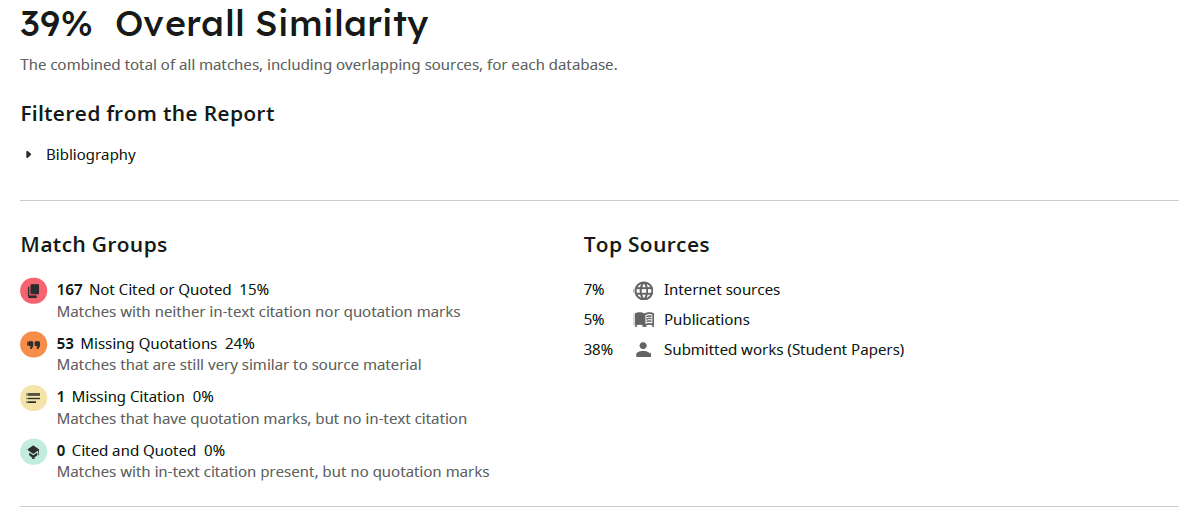
\includegraphics[width=\textwidth]{images/turnitin1.png}
\end{figure}

\begin{figure}[H]
    \centering
    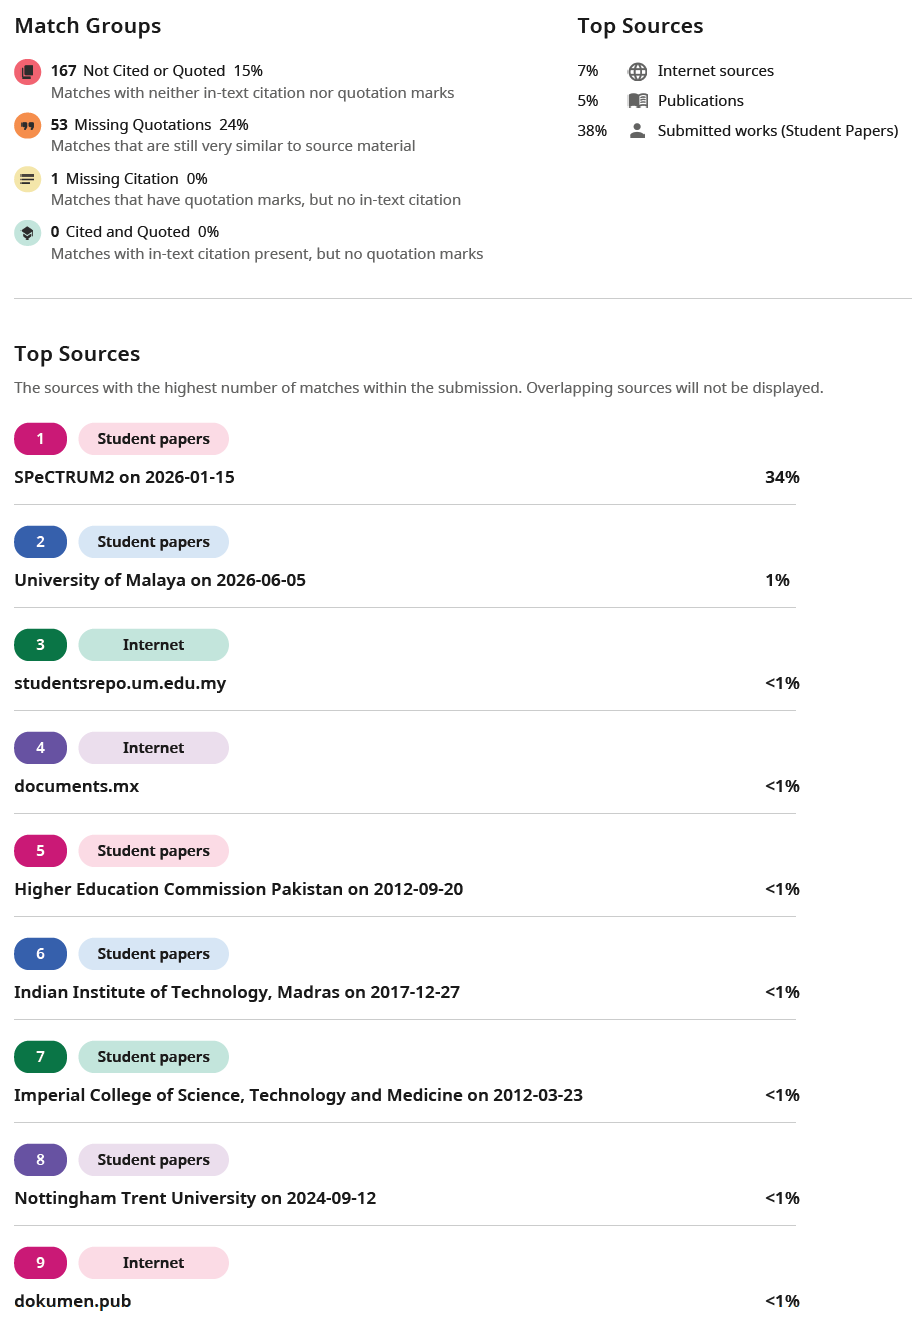
\includegraphics[width=\textwidth]{images/turnitin2.png}
\end{figure}

\clearpage

% ============================================================
% APPENDIX B
% ============================================================
\chapter*{Appendix B -- AI Use Declaration Form for Assessment}
\addcontentsline{toc}{chapter}{Appendix B -- AI Use Declaration Form for Assessment}

{\setlength{\parindent}{0pt}
\noindent\raisebox{0cm}{\framebox(14,14){}}\quad I hereby declare that part of this submitted assessment contains contributions generated through the use of AI software, and that such use is consistent with the permissible usage stated in the AI Use in T\&L Activities Declaration Form, the assignment briefing, or the assessment guidelines, and is in line with good academic practice.

\vspace{1em}

\noindent The content submitted may still be regarded as my own work. I understand that as long as my use falls within the category of ``permissible use'' as defined in the summary/guidelines for the assessment, this declaration will not have any direct impact on the grade awarded.

\vspace{1em}

\noindent I acknowledge the use of software for the following purposes [e.g., preparation of thesis writing]:}

\vspace{1em}

% ---- TABLE PART 1 (row i) ----
\noindent\begin{tabular}{|p{0.07\textwidth}|p{0.25\textwidth}|p{0.55\textwidth}|}
\hline
\textbf{NO.} & \textbf{ITEM} & \textbf{USAGE} \\
\hline
(i) &
Generating ideas or structural suggestions, for assistance in understanding core concepts, or other essential preliminary activities. &
\textbf{Level 2} --- Perplexity.ai was used during the early research planning phase to brainstorm potential engineering application ideas for extending the validated PEC cylinder finite element solver. This led to the identification of LSPR biosensing as the target application domain. All subsequent technical understanding was developed independently through reading peer-reviewed literature from Google Scholar.\newline
\texttt{perplexity.ai}\newline\newline
\textbf{Level 2} --- Gemini (gemini.google.com) was used for concept checking during the literature review phase. When peer-reviewed papers contained highly technical language, Gemini provided simplified explanations and analogies to aid understanding. No Gemini-generated text was included in the thesis manuscript.\newline
\texttt{gemini.google.com}\newline\newline
\textbf{Level 2} --- Claude (claude.ai) was used for concept checking and brainstorming during solver development, including understanding FEniCSx/DOLFINx API behaviour, exploring solutions to finite element implementation issues, suggesting thesis chapter structures, and understanding ParaView features for post-processing simulation outputs. All research decisions and conclusions were made independently by the author.\newline
\texttt{claude.ai} \\
\hline
\end{tabular}

\vspace{0pt}

% ---- TABLE PART 2 (rows ii to v) ----
\noindent\begin{tabular}{|p{0.07\textwidth}|p{0.25\textwidth}|p{0.55\textwidth}|}
\hline
\textbf{NO.} & \textbf{ITEM} & \textbf{USAGE} \\
\hline
(ii) &
Rewriting, rephrasing, and/or paraphrasing parts of this assessment. &
\textbf{Level 2} --- Gemini (gemini.google.com) and Claude (claude.ai) were used for specific grammar checking and paraphrasing tasks on author-written content to improve sentence clarity and ensure formal academic reporting style. The original content, ideas, technical substance, and intellectual contributions are entirely the author's own.\newline
\texttt{gemini.google.com}\newline
\texttt{claude.ai} \\
\hline
(iii) &
Producing elements other than the submitted assessment itself, such as full-sentence/paragraph writing, image/audio/video generation, or data analysis. &
\textbf{Level 2} --- Claude (claude.ai) was used for the specific task of converting author-written draft content into properly structured \LaTeX{} markup, including formatting equations, tables, figures, and citation commands. The written content, research findings, and all intellectual contributions are entirely the author's own.\newline
\texttt{claude.ai} \\
\hline
(iv) &
Using AI mandatorily as a compulsory component of an assignment to produce, evaluate, compare, or critique AI outputs. &
N/A \\
\hline
(v) &
Others &
N/A \\
\hline
\end{tabular}

\vspace{2em}

{\setlength{\parindent}{0pt}
\noindent \textit{If no AI was used:}

\vspace{0.8em}

\noindent\raisebox{0cm}{\framebox(14,14){}}\quad I hereby declare that no AI software was used in completing this assessment.}

\vspace{3em}

\noindent
\begin{tabular}{p{0.35\textwidth} p{0.05\textwidth} p{0.45\textwidth}}
Candidate's Signature & : & \underline{\hspace{7cm}} \\[1.2em]
Date                  & : & \underline{\hspace{7cm}} \\
\end{tabular}